\documentclass{article}\usepackage[]{graphicx}\usepackage[]{color}
%% maxwidth is the original width if it is less than linewidth
%% otherwise use linewidth (to make sure the graphics do not exceed the margin)
\makeatletter
\def\maxwidth{ %
  \ifdim\Gin@nat@width>\linewidth
    \linewidth
  \else
    \Gin@nat@width
  \fi
}
\makeatother

\definecolor{fgcolor}{rgb}{0.345, 0.345, 0.345}
\newcommand{\hlnum}[1]{\textcolor[rgb]{0.686,0.059,0.569}{#1}}%
\newcommand{\hlstr}[1]{\textcolor[rgb]{0.192,0.494,0.8}{#1}}%
\newcommand{\hlcom}[1]{\textcolor[rgb]{0.678,0.584,0.686}{\textit{#1}}}%
\newcommand{\hlopt}[1]{\textcolor[rgb]{0,0,0}{#1}}%
\newcommand{\hlstd}[1]{\textcolor[rgb]{0.345,0.345,0.345}{#1}}%
\newcommand{\hlkwa}[1]{\textcolor[rgb]{0.161,0.373,0.58}{\textbf{#1}}}%
\newcommand{\hlkwb}[1]{\textcolor[rgb]{0.69,0.353,0.396}{#1}}%
\newcommand{\hlkwc}[1]{\textcolor[rgb]{0.333,0.667,0.333}{#1}}%
\newcommand{\hlkwd}[1]{\textcolor[rgb]{0.737,0.353,0.396}{\textbf{#1}}}%
\let\hlipl\hlkwb

\usepackage{framed}
\makeatletter
\newenvironment{kframe}{%
 \def\at@end@of@kframe{}%
 \ifinner\ifhmode%
  \def\at@end@of@kframe{\end{minipage}}%
  \begin{minipage}{\columnwidth}%
 \fi\fi%
 \def\FrameCommand##1{\hskip\@totalleftmargin \hskip-\fboxsep
 \colorbox{shadecolor}{##1}\hskip-\fboxsep
     % There is no \\@totalrightmargin, so:
     \hskip-\linewidth \hskip-\@totalleftmargin \hskip\columnwidth}%
 \MakeFramed {\advance\hsize-\width
   \@totalleftmargin\z@ \linewidth\hsize
   \@setminipage}}%
 {\par\unskip\endMakeFramed%
 \at@end@of@kframe}
\makeatother

\definecolor{shadecolor}{rgb}{.97, .97, .97}
\definecolor{messagecolor}{rgb}{0, 0, 0}
\definecolor{warningcolor}{rgb}{1, 0, 1}
\definecolor{errorcolor}{rgb}{1, 0, 0}
\newenvironment{knitrout}{}{} % an empty environment to be redefined in TeX

\usepackage{alltt}%[final]
\setcounter{secnumdepth}{3}
% if you need to pass options to natbib, use, e.g.:
% \PassOptionsToPackage{numbers, compress}{natbib}
% before loading nips_2016
%
% to avoid loading the natbib package, add option nonatbib:
% \usepackage[nonatbib]{nips_2016}

%\usepackage{nips_2016}

% to compile a camera-ready version, add the [final] option, e.g.:
%\usepackage[final]{nips_2016}
\usepackage{amsmath}
\usepackage[utf8]{inputenc} % allow utf-8 input
\usepackage[T1]{fontenc}    % use 8-bit T1 fonts
\usepackage{hyperref}       % hyperlinks
\usepackage{url}            % simple URL typesetting
\usepackage{booktabs}       % professional-quality tables
\usepackage{amsfonts}       % blackboard math symbols
\usepackage{nicefrac}       % compact symbols for 1/2, etc.
\usepackage{microtype}      % microtypography
\usepackage{float}
\usepackage{amssymb}
\usepackage{amsthm}
\usepackage{color,soul}
\usepackage{amsmath}
\usepackage{algorithm}
\usepackage[noend]{algpseudocode}
\usepackage[margin=1.5in]{geometry}
\usepackage[english]{babel}
\usepackage{graphicx}
\usepackage{longtable}

\newtheorem{theorem}{Theorem}[section]
\newtheorem{lemma}[theorem]{Lemma}
\newtheorem{proposition}[theorem]{Proposition}
\newtheorem{corollary}[theorem]{Corollary}
\theoremstyle{definition}
\newtheorem{definition}{Definition}[section]

% Code defs from jss
\newcommand\code{\@codex}
\def\@codex#1{{\normalfont\ttfamily\hyphenchar\font=-1 #1}}
%%\let\code=\texttt
\let\proglang=\textsf
\newcommand{\pkg}[1]{{\fontseries{b}\selectfont #1}}


%\theoremstyle{definition}
%\newtheorem{definition}{Definition}[section]


\makeatletter
\def\BState{\State\hskip-\ALG@thistlm}
\makeatother

\title{Time Series Methods in the R package \pkg{mlr}}

% The \author macro works with any number of authors. There are two
% commands used to separate the names and addresses of multiple
% authors: \And and \AND.
%
% Using \And between authors leaves it to LaTeX to determine where to
% break the lines. Using \AND forces a line break at that point. So,
% if LaTeX puts 3 of 4 authors names on the first line, and the last
% on the second line, try using \AND instead of \And before the third
% author name.

\author{
  Steve Bronder \\
  %Quantitative Methods of the Social Sciences\\
  %Columbia University\\
  %New York City, NY 10027 \\
  \texttt{sab2287@columbia.edu} \\
  %% examples of more authors test etst
   %Department of Computer Science \\
   %Columbia University\\
   %New York City, NY 10027 \\
  %% \AND
  %% Coauthor \\
  %% Affiliation \\
  %% Address \\
  %% \texttt{email} \\
  %% \And
  %% Coauthor \\
  %% Affiliation \\
  %% Address \\
  %% \texttt{email} \\
  %% \And
  %% Coauthor \\
  %% Affiliation \\
  %% Address \\
  %% \texttt{email} \\
}
\IfFileExists{upquote.sty}{\usepackage{upquote}}{}
\begin{document}
% \nipsfinalcopy is no longer used

\maketitle

\begin{abstract}
The \pkg{mlr} package is a unified interface for machine learning tasks such as classification, regression, cluster analysis, and survival analysis. \pkg{mlr} handles the data pipeline of pre-processing, resampling, model selection, model tuning, ensembling, and prediction. This paper details new methods for developing time series  models in \pkg{mlr}. It includes standard and novel tools such as auto-regressive and LambertW transform data generating processes, fixed and growing window cross validation, and forecasting models in the context of univariate and multivariate time series. Examples from forecasting competitions will be given in order to demonstrate the benefits of a unified framework for machine learning and time series.
  \end{abstract}

\section{Introduction}
There has been a rapid developement in time series methods over the last 25 years ~\cite{Hyndman25}. Time series models have not only become more common, but more complex. The \proglang{R} language ~\cite{Rbase} has a large task view with many packages available for forecasting and time series methods. However, without a standard framework, many packages have their own sub-culture of style, syntax, and output. The \pkg{mlr} ~\cite{mlr} package, short for Machine Learning in R, works to give a strong syntatic framework for the modeling pipeline. By automating many of the standard tools in machine learning such as preprocessing and cross validation, \pkg{mlr} reduces error in the modeling process that is derived from the user. 

While there are some time series methods available in \pkg{caret} ~\cite{caret}, development of forecasting models in \pkg{caret} is difficult due to computational constraints and design choices. The highly modular structure of \pkg{mlr} makes it the best choice for implementing time series methods and models. This paper will show how using \pkg{mlr}'s strong syntatic structure allows for time series packages such as \pkg{forecast} ~\cite{HyndForecast} and \pkg{rugarch} ~\cite{rugarch} to use machine learning methedologies such as automated parameter tuning, data preprocessing, model blending, cross validation, performance evaluation, and parallel processing techniques for decreasing model build time.

\section{Forecasting Example with the M4 Competition}
\label{sec:m4data}

Professional forecasters attempt to predict the future of a series based on its past values. Forecasting can be used in a wide range of tasks including forecasting stock prices, ~\cite{GRANGER19923}, weather patterns ~\cite{MurphymeteoForecast}, international conficts ~\cite{Chadefaux01012014}, and earthquakes ~\cite{earthquakeYegu}. In order to evaluate \pkg{mlr}'s forecasting framework we need a large set of possible time series to make sure our methods generalize well.\footnote{Very goofy sentence need to fix}

The Makridakis competitions ~\cite{Makridakis2000451} are forecasting challenges organized by the International Institute of Forecasters and led by Spyros Makridakis to evaluate and compare the accuracy of forecasting methods. The most recent of the competitions, the M4 competition, contains 10,000 time series on a yearly, quarterly, monthly, and daily frequency in areas such as finance, macroeconomics, microeconomics, and industry. For our purposes we will look at two particular daily financial series, one with 9136 observations from April 10th, 1971 to April 13th, 1996 and another with 6742 observations from January 7th, 1981 to June 23rd, 1999. Each series must be forecast 328 and 242 periods into the future, respectively.



\begin{knitrout}
\definecolor{shadecolor}{rgb}{0.969, 0.969, 0.969}\color{fgcolor}

{\centering 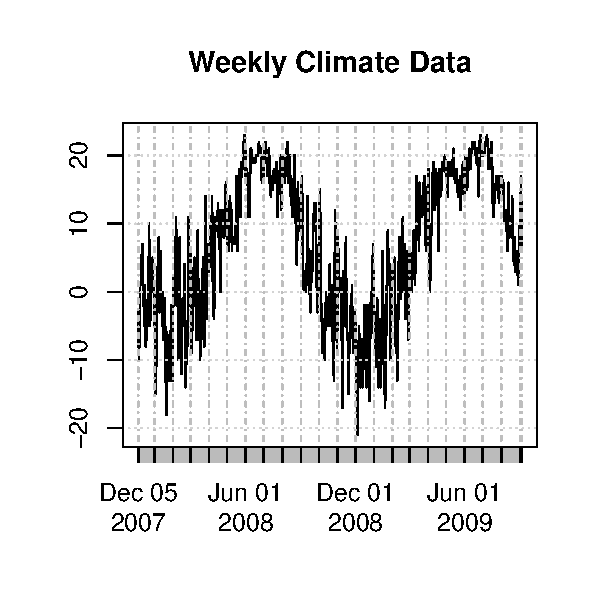
\includegraphics[width=\maxwidth]{figure/get_dat-1} 

}




{\centering 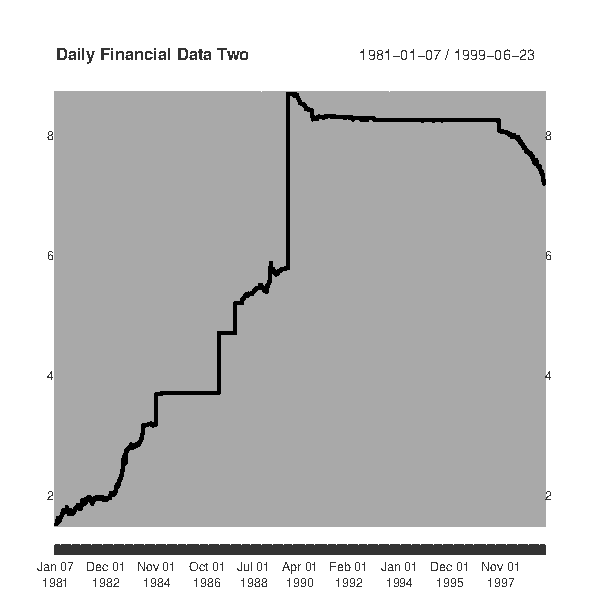
\includegraphics[width=\maxwidth]{figure/get_dat-2} 

}



\end{knitrout}

These two series were chosen for their large time features and stark contrast.\footnote{I think it would be better to just use one series for examples, and actually train / test over all of M4 later} Our data set should be large enough that the tuning method can take multiple windows of the data. Some series in M4 only contain 12 observations, which is not enough data to accurately train a model. These two time series were chosen as they are the two largest ones in the M4 competitions data set. We can see figure one is what most people imagine when they think of a time series. Figure two shows a series which appears to have a sort of step feature. The stark difference between the time process of the two series will allow us to investigate whether the methods in \pkg{mlr}'s forecasting framework can find the appropriate model. The data can be found in the package \pkg{M4comp} ~\cite{m4comp} under sets `M4[28]` and `M4[29]. 

\section{Forecasting Tasks}
\label{sec:task}

\pkg{mlr} provides uses the S3 object system to clearly define a predictive modeling task. Tasks contain the data and other relevant information such as the task id and which variable you are targeting for supervised learning problems. Forecasting tasks are handled in \pkg{mlr} by the function \code{makeForecastRegrTask()}. The forecasting task inherets from \code{makeRegrTask}, but has two noticable differences in parameters.

\begin{itemize}
\item[data:] Instead of a data frame, an xts object from \pkg{xts} ~\cite{xts} containing the time series.
\item[frequency:] An integer with the number of periods your time series contains. For example, daily data with a weekly periodicity has a frequency of 7 while daily data with a yearly periodicity has a frequency of 365.
\end{itemize}

\begin{knitrout}
\definecolor{shadecolor}{rgb}{0.969, 0.969, 0.969}\color{fgcolor}\begin{kframe}
\begin{alltt}
\hlkwd{library}\hlstd{(mlr)}
\end{alltt}


{\ttfamily\noindent\itshape\color{messagecolor}{\#\# Loading required package: ParamHelpers}}\begin{alltt}
\hlstd{Fin.task1} \hlkwb{=} \hlkwd{makeForecastRegrTask}\hlstd{(}\hlkwc{id} \hlstd{=} \hlstr{"M4 Finance Data One"}\hlstd{,}
                                 \hlkwc{data} \hlstd{= m4Train1,}
                                 \hlkwc{target} \hlstd{=} \hlstr{"target_var"}\hlstd{,}
                                 \hlkwc{frequency} \hlstd{=} \hlnum{7L}\hlstd{)}
\hlstd{Fin.task1}
\end{alltt}
\begin{verbatim}
## Task: M4 Finance Data One
## Type: regr
## Observations: 9136
## Dates:
##  Start: 1971-04-10 
##  End: 1996-04-13
## Frequency: 7
## Features:
## numerics  factors  ordered 
##        1        0        0 
## Missings: FALSE
## Has weights: FALSE
## Has blocking: FALSE
\end{verbatim}
\end{kframe}
\end{knitrout}

\section{Building a forecast learner}

The \code{makeLearner()} function provides a structured model building framework to the 7 forecasting models currently implimented in \pkg{mlr}. As an example, we will build a simple AutoRegressive Integrated Moving Average (ARIMA) model. The ARIMA model is of the form

\begin{equation}
y_t \sim \alpha + \beta_1 \Delta_d y_{t-1} ... \beta_p \Delta_d y_{t-p} + \phi_1 \epsilon_{t-1} + ... + \phi_q \epsilon_{t-q} + \epsilon_t
\end{equation}

\begin{equation}
y_t \sim \alpha + \sum_{i=1}^p \beta_i \Delta_d y_{t-i} + \sum_{i=1}^q \phi_i \epsilon_{t-i} +\epsilon_t
\end{equation}

In equation three, $\alpha$ is a constant, $\beta_p$ is the coefficient associated with the lagged observations of $y$ with $\Delta_d$ being the $d$th difference operator. The coefficient for the one step forecast error $\epsilon_{t-q}$ is $\phi_q$. ARIMA is one of the most well known forecasting models and is avaible in mlr along with models such as BATS, TBATS, THIEF ~\cite{thief}, ETS, several GARCH variants, and autoregressive neural networks. In addition, preprocessing features have been added to allow arbitrary supervised machine learning models to be used in the context of forecasting.

To impliment this model we use \code{makeLearner()}, supplying the class of learner, order, the number of steps to forecast, and any additional arguments to be passed to \code{Arima} for \pkg{forecast}. 

\begin{knitrout}
\definecolor{shadecolor}{rgb}{0.969, 0.969, 0.969}\color{fgcolor}\begin{kframe}
\begin{alltt}
\hlstd{arm} \hlkwb{=} \hlkwd{makeLearner}\hlstd{(}\hlstr{"fcregr.Arima"}\hlstd{,} \hlkwc{order} \hlstd{=} \hlkwd{c}\hlstd{(}\hlnum{2L}\hlstd{,}\hlnum{0L}\hlstd{,}\hlnum{1L}\hlstd{),} \hlkwc{h} \hlstd{=} \hlnum{328L}\hlstd{,} \hlkwc{include.mean} \hlstd{=} \hlnum{FALSE}\hlstd{)}
\hlstd{arm}
\end{alltt}
\begin{verbatim}
## Learner fcregr.Arima from package forecast
## Type: regr
## Name: AutoRegressive Integrated Moving Average; Short name: Arima
## Class: fcregr.Arima
## Properties: numerics,ts
## Predict-Type: response
## Hyperparameters: order=2,0,1,h=328,include.mean=FALSE
\end{verbatim}
\end{kframe}
\end{knitrout}

To train the model we simply call train, supplying the model and task.

\begin{knitrout}
\definecolor{shadecolor}{rgb}{0.969, 0.969, 0.969}\color{fgcolor}\begin{kframe}
\begin{alltt}
\hlstd{trainArima} \hlkwb{=} \hlkwd{train}\hlstd{(arm, Fin.task1 )}
\hlstd{trainArima}
\end{alltt}
\begin{verbatim}
## Model for learner.id=fcregr.Arima; learner.class=fcregr.Arima
## Trained on: task.id = M4 Finance Data One; obs = 9136; features = 1
## Hyperparameters: order=2,0,1,h=328,include.mean=FALSE
\end{verbatim}
\end{kframe}
\end{knitrout}

While ARIMA is one of the most well known time series models, the order selection process can be subjective and difficult for users. One of the first proposals for automatic order selection comes from ~\cite{hannanOrder} where innovations are obtained by fitting high order autoregressive model to the data and then computing the likelihood of potential models through a series of standard regresssions. Proprietary algorithms from software such as \proglang{Forecast Pro} ~\cite{forecastpro} and \proglang{Autobox} ~\cite{reillyautobox} are well known and have performed to high standards in competitions such as the M3 forecasting competition ~\cite{Makridakis2000451}. One of the most well known R packages for automated forecast is \pkg{forecast} ~\cite{HyndForecast} which contains several methods for automated forecasting including exponential smoothing based methods and step-wise algorithms for forecasting with ARIMA models.

Forecasting in \pkg{mlr} takes a machine learning approach, creating a parameter set for a given model and using an optimization method to search over the parameter space. To do this, we will use a windowing resampling scheme to train over the possible models.

\section{Resampling with Time}

Resampling schemes such as cross-validation, bootstrapping, etc. are common in machine learning for dealing with the bias-variance tradeoff ~\cite{Friedman1997} ~\cite{rodriguezkfold}. When their is a time component to the data, windowing schemes are useful in allowing a valid resampling scheme while still maintaining the time properties of the series.\footnote{crap}. Figure one gives an example of what fixed and growing windows look like. Given a horizon and initial starting point the window slides forward one step each time while either shifting in the fixed case or enlarging by one in the growing case. Growing and fixed window resampling such as from ~\cite{hyndman2014forecasting} are now available in the \code{resampling()} function of \pkg{mlr}. 

\begin{figure}[ht]
\caption{Resampling with a window scheme as exampled by caret ~\cite{windowingcaret} }
  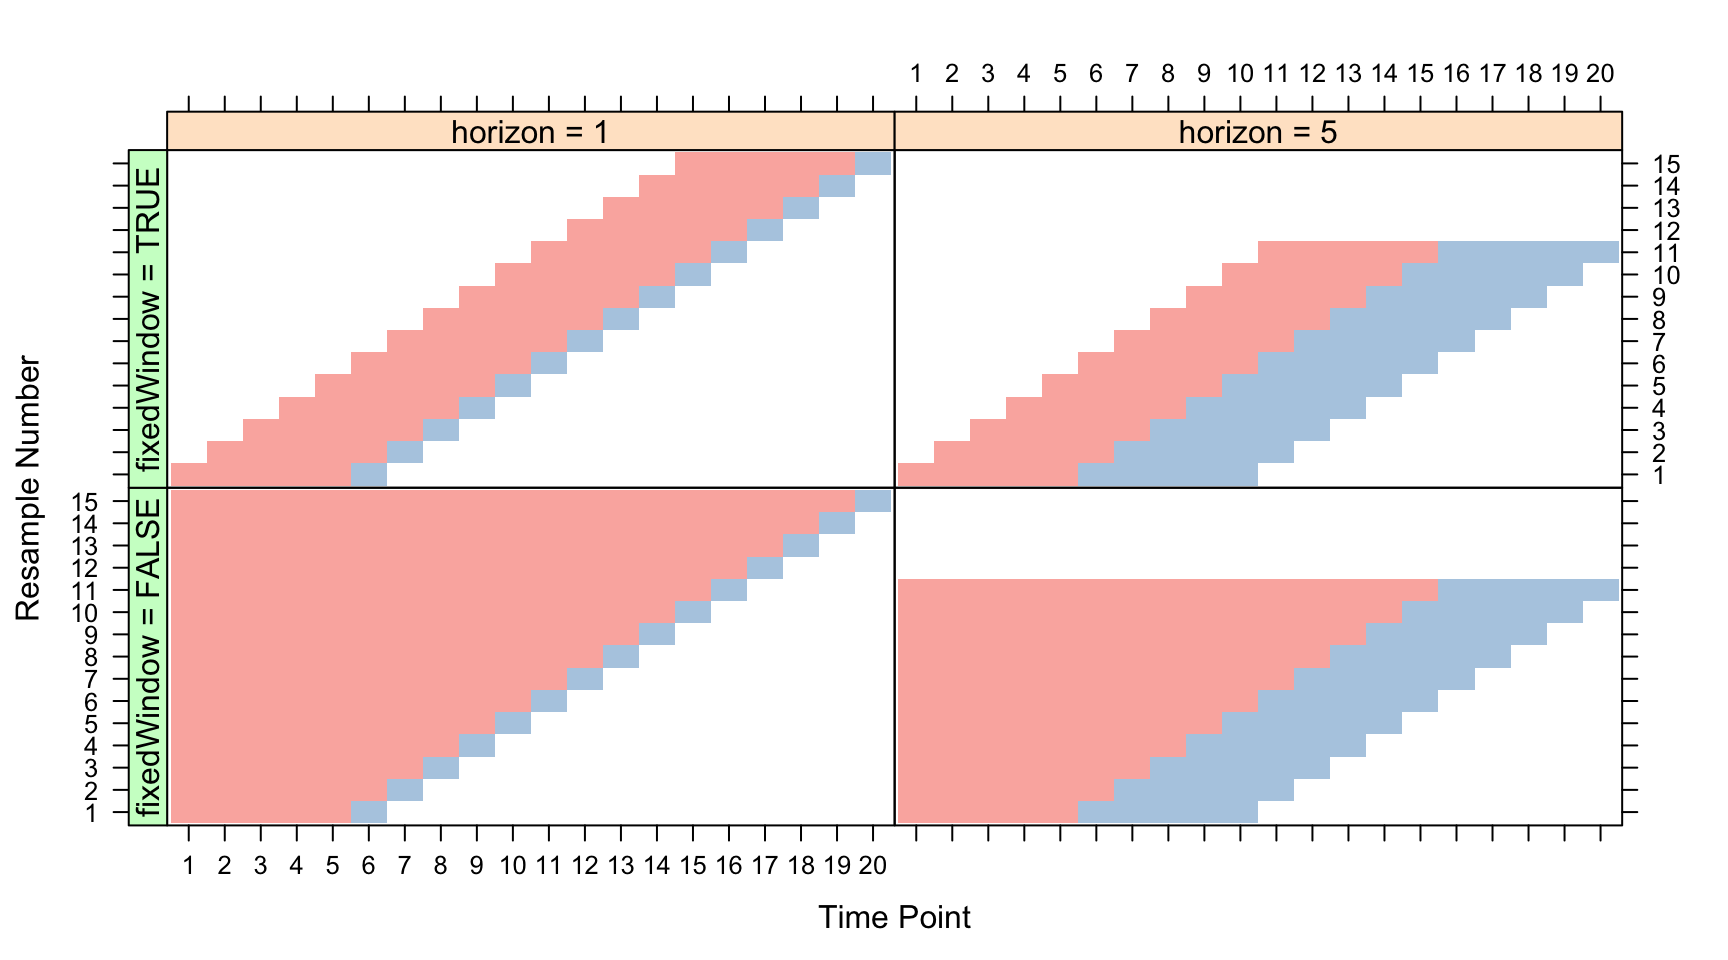
\includegraphics[scale = .2]{windowing_pic_caret}
  \centering
\end{figure}
%% Note: If there is markup in \(sub)section, then it has to be escape as above.
\newpage

A windowing resampling process is created in the function \code{makeResampleDesc()} by supplying the resampling type, horizon, initial window, the length of the series, and an optional parameter to skip over some windows for the sake of time.

\begin{knitrout}
\definecolor{shadecolor}{rgb}{0.969, 0.969, 0.969}\color{fgcolor}\begin{kframe}
\begin{alltt}
\hlstd{resampDesc} \hlkwb{=} \hlkwd{makeResampleDesc}\hlstd{(}\hlstr{"GrowingCV"}\hlstd{,} \hlkwc{horizon} \hlstd{=} \hlnum{328L}\hlstd{,}
                               \hlkwc{initialWindow} \hlstd{=} \hlnum{6000L}\hlstd{,}
                               \hlkwc{size} \hlstd{=} \hlkwd{nrow}\hlstd{(}\hlkwd{getTaskData}\hlstd{(Fin.task1)),} \hlkwc{skip} \hlstd{=} \hlnum{100L}\hlstd{)}
\hlstd{resampDesc}
\end{alltt}
\begin{verbatim}
## Window description:
##  growing with 28 iterations:
##  6000 observations in initial window and 328 horizon.
## Predict: test
## Stratification: FALSE
\end{verbatim}
\end{kframe}
\end{knitrout}

To make a parameter set to tune over \pkg{mlr} uses \pkg{ParamHelpers} ~\cite{paramhelper}. For this example we tune over the entire grid space by setting our tune control to a grid search. 
\begin{knitrout}
\definecolor{shadecolor}{rgb}{0.969, 0.969, 0.969}\color{fgcolor}\begin{kframe}
\begin{alltt}
\hlstd{parSet} \hlkwb{=} \hlkwd{makeParamSet}\hlstd{(}
  \hlkwd{makeIntegerVectorParam}\hlstd{(}\hlkwc{id} \hlstd{=} \hlstr{"order"}\hlstd{,}
                         \hlkwc{len} \hlstd{=} \hlnum{3}\hlstd{,}
                         \hlkwc{lower} \hlstd{=} \hlkwd{c}\hlstd{(}\hlnum{10}\hlstd{,}\hlnum{0}\hlstd{,}\hlnum{3}\hlstd{),}
                         \hlkwc{upper} \hlstd{=} \hlkwd{c}\hlstd{(}\hlnum{14}\hlstd{,}\hlnum{3}\hlstd{,}\hlnum{6}\hlstd{),}
                         \hlkwc{tunable} \hlstd{=} \hlnum{TRUE}\hlstd{),}
  \hlkwd{makeIntegerVectorParam}\hlstd{(}\hlkwc{id} \hlstd{=} \hlstr{"seasonal"}\hlstd{,}
                         \hlkwc{len} \hlstd{=} \hlnum{3}\hlstd{,}
                         \hlkwc{lower} \hlstd{=} \hlkwd{c}\hlstd{(}\hlnum{0}\hlstd{,}\hlnum{0}\hlstd{,}\hlnum{0}\hlstd{),}
                         \hlkwc{upper} \hlstd{=} \hlkwd{c}\hlstd{(}\hlnum{3}\hlstd{,}\hlnum{3}\hlstd{,}\hlnum{3}\hlstd{),}
                         \hlkwc{tunable} \hlstd{=} \hlnum{TRUE}\hlstd{),}
  \hlkwd{makeLogicalParam}\hlstd{(}\hlkwc{id} \hlstd{=} \hlstr{"include.mean"}\hlstd{,}
                   \hlkwc{default} \hlstd{=} \hlnum{FALSE}\hlstd{,}
                   \hlkwc{tunable} \hlstd{=} \hlnum{TRUE}\hlstd{),}
  \hlkwd{makeLogicalParam}\hlstd{(}\hlkwc{id} \hlstd{=} \hlstr{"include.drift"}\hlstd{,}
                   \hlkwc{default} \hlstd{=} \hlnum{FALSE}\hlstd{,}
                   \hlkwc{tunable} \hlstd{=} \hlnum{TRUE}\hlstd{),}
  \hlkwd{makeNumericParam}\hlstd{(}\hlkwc{id} \hlstd{=} \hlstr{"h"}\hlstd{,}
                   \hlkwc{default} \hlstd{=} \hlnum{328}\hlstd{,}
                   \hlkwc{tunable} \hlstd{=} \hlnum{FALSE}\hlstd{,}
                   \hlkwc{lower} \hlstd{=} \hlnum{328}\hlstd{,}
                   \hlkwc{upper} \hlstd{=} \hlnum{328}\hlstd{)}
\hlstd{)}

\hlcom{#Specify tune by grid estimation}
\hlstd{ctrl} \hlkwb{=} \hlkwd{makeTuneControlGrid}\hlstd{()}
\end{alltt}
\end{kframe}
\end{knitrout}

Using \code{tuneParams()} the model is tuned for the task using the specified resampling scheme, parameter set, tune control, and measure. For this tuning task we use MASE ~\cite{Hyndman2006} as a measure of performance \footnote{Models with a seasonal difference $> 0$ may be favorably biased as we use the non-seasonal MASE score}.

\begin{knitrout}
\definecolor{shadecolor}{rgb}{0.969, 0.969, 0.969}\color{fgcolor}\begin{kframe}
\begin{alltt}
\hlcom{#}
\hlstd{res} \hlkwb{=} \hlkwd{tuneParams}\hlstd{(}\hlstr{"fcregr.Arima"}\hlstd{,} \hlkwc{task} \hlstd{= Fin.task1,} \hlkwc{resampling} \hlstd{= resampDesc,}
                 \hlkwc{par.set} \hlstd{= parSet,} \hlkwc{control} \hlstd{= ctrl,} \hlkwc{measures} \hlstd{= mase)}

\hlstd{res}
\end{alltt}
\end{kframe}
\end{knitrout}

The best model's parameters are extracted using \code{setHyperPars()} and the best model is passed to \code{train()} to go over the full data set.

\begin{knitrout}
\definecolor{shadecolor}{rgb}{0.969, 0.969, 0.969}\color{fgcolor}\begin{kframe}
\begin{alltt}
\hlstd{lrn} \hlkwb{=} \hlkwd{setHyperPars}\hlstd{(}\hlkwd{makeLearner}\hlstd{(}\hlstr{"fcregr.Arima"}\hlstd{),} \hlkwc{par.vals} \hlstd{= res}\hlopt{$}\hlstd{x)}
\hlstd{m} \hlkwb{=} \hlkwd{train}\hlstd{(lrn, Timeregr.task)}
\end{alltt}
\end{kframe}
\end{knitrout}

To make predictions for our test set we simply pass our model, task, and test data to \code{predict()}

\begin{knitrout}
\definecolor{shadecolor}{rgb}{0.969, 0.969, 0.969}\color{fgcolor}\begin{kframe}
\begin{alltt}
\hlkwd{predict}\hlstd{(m,} \hlkwc{task} \hlstd{= Fin.task1,} \hlkwc{newdata} \hlstd{= m4Test1)}
\end{alltt}
\end{kframe}
\end{knitrout}

\newpage
%\small
\bibliography{thesisbib}{}
\bibliographystyle{plain}

\end{document}
